\documentclass[a4paper,11pt]{article}
\usepackage{amsmath,amsthm,amsfonts,amssymb,amscd,amstext,vmargin,graphics,graphicx,tabularx,multicol} 
\usepackage[francais]{babel}
\usepackage[utf8]{inputenc}  
\usepackage[T1]{fontenc} 
\usepackage{pstricks-add,tikz,tkz-tab,variations}
\usepackage[autolanguage,np]{numprint} 

\setmarginsrb{1.5cm}{0.5cm}{1cm}{0.5cm}{0cm}{0cm}{0cm}{0cm} %Gauche, haut, droite, haut
\newcounter{numexo}
\newcommand{\exo}[1]{\stepcounter{numexo}\noindent{\bf Exercice~\thenumexo} : \marginpar{\hfill /#1}}
\reversemarginpar


\newcounter{enumtabi}
\newcounter{enumtaba}
\newcommand{\q}{\stepcounter{enumtabi} \theenumtabi.  }
\newcommand{\qa}{\stepcounter{enumtaba} (\alph{enumtaba}) }
\newcommand{\initq}{\setcounter{enumtabi}{0}}
\newcommand{\initqa}{\setcounter{enumtaba}{0}}

\newcommand{\be}{\begin{enumerate}}
\newcommand{\ee}{\end{enumerate}}
\newcommand{\bi}{\begin{itemize}}
\newcommand{\ei}{\end{itemize}}
\newcommand{\bp}{\begin{pspicture*}}
\newcommand{\ep}{\end{pspicture*}}
\newcommand{\bt}{\begin{tabular}}
\newcommand{\et}{\end{tabular}}
\renewcommand{\tabularxcolumn}[1]{>{\centering}m{#1}} %(colonne m{} centrée, au lieu de p par défault) 
\newcommand{\tnl}{\tabularnewline}

\newcommand{\bmul}[1]{\begin{multicols}{#1}}
\newcommand{\emul}{\end{multicols}}

\newcommand{\trait}{\noindent \rule{\linewidth}{0.2mm}}
\newcommand{\hs}[1]{\hspace{#1}}
\newcommand{\vs}[1]{\vspace{#1}}

\newcommand{\N}{\mathbb{N}}
\newcommand{\Z}{\mathbb{Z}}
\newcommand{\R}{\mathbb{R}}
\newcommand{\C}{\mathbb{C}}
\newcommand{\Dcal}{\mathcal{D}}
\newcommand{\Ccal}{\mathcal{C}}
\newcommand{\mc}{\mathcal}

\newcommand{\vect}[1]{\overrightarrow{#1}}
\newcommand{\ds}{\displaystyle}
\newcommand{\eq}{\quad \Leftrightarrow \quad}
\newcommand{\vecti}{\vec{\imath}}
\newcommand{\vectj}{\vec{\jmath}}
\newcommand{\Oij}{(O;\vec{\imath}, \vec{\jmath})}
\newcommand{\OIJ}{(O;I,J)}


\newcommand{\reponse}[1][1]{%
\multido{}{#1}{\makebox[\linewidth]{\rule[0pt]{0pt}{20pt}\dotfill}
}}

\newcommand{\titre}[5] 
% #1: titre #2: haut gauche #3: bas gauche #4: haut droite #5: bas droite
{
\noindent #2 \hfill #4 \\
#3 \hfill #5

\vspace{-1.6cm}

\begin{center}\rule{6cm}{0.5mm}\end{center}
\vspace{0.2cm}
\begin{center}{\large{\textbf{#1}}}\end{center}
\begin{center}\rule{6cm}{0.5mm}\end{center}
}



\begin{document}
\pagestyle{empty}

\titre{Correction du contrôle  : Trigonométrie et Théorème de Pythagore}{Nom}{Prénom}{Date}{Classe}
\vspace*{0.5cm}

\exo{1.5} Dans chaque cas, donner la valeur arrondie au degré de $x$.\\
\initqa \qa $sin(x)=0,65$ \hspace*{0.5cm} \qa $tan(x)=18$  \hspace*{0.5cm} \qa $cos(x)=\dfrac{7}{9}$ \\
\color{red}
\initqa \qa $x \approx 41$° \hspace*{1.5cm} \qa  $x \approx 87$° \hspace*{1.5cm} \qa  $x \approx 39$° \\
\color{black}
\vspace*{0.25cm}

\exo{3} Calculer la longueur RS arrondie au millimètre.
\begin{center}
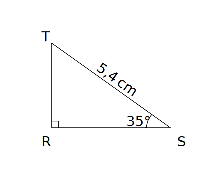
\includegraphics[scale=1.4]{trigo1.eps} 
\end{center}
\vspace*{0.25cm}

\color{red}
\textbf{CORRECTION :}

Le triangle RST est rectangle en R. \\
Je connais l'angle $\widehat{TSR}$ et l'hypoténuse du triangle [TS] et je cherche la longueur du côté adjacent([RS])\\

J'utilise donc la formule du cosinus :

\bmul{2}

$cos \widehat{TSR} = \dfrac{\textrm{côté adjacent}}{\textrm{hypoténuse}} $\\

$cos \widehat{TSR} = \dfrac{RS}{TS}$\\

$cos \textrm{35°} = \dfrac{RS}{5,4}$\\

\columnbreak

 $ RS = 5,4 \times cos \textrm{35°}$\\

\fbox{$RS \approx 4,4 cm$ }

\emul


\color{black}
\exo{4.5}

\includegraphics[scale=1.2]{trigo2.eps} \\

\noindent \initqa \qa Calculer la mesure arrondie au degré de l'angle $\widehat{MPN}$.\\


\color{red}
\textbf{CORRECTION :}

\initqa \qa Le triangle NMP est rectangle en M. \\
Je connais la longueur du côté adjacent([MP]) et la longueur du côté opposé [NM] et je cherche l'angle $\widehat{MPN}$\\

J'utilise donc la formule du tangente :

\bmul{2}

$tan \widehat{MPN} = \dfrac{\textrm{côté opposé}}{\textrm{côté adjacent}} $\\

$tan \widehat{MPN} = \dfrac{NM}{MP}$\\

$tan \widehat{MPN} = \dfrac{4,3}{6,5}$\\

\columnbreak

 $ \widehat{MPN} = arctan(\dfrac{4,3}{6,5})$\\

\fbox{$\widehat{MPN}  \approx 33° $ }

\emul


\color{black}

\newpage

\qa En déduire la mesure arrondie au degré de l'angle $\widehat{MNP}$.\\

\color{red}
\textbf{CORRECTION :}

2 propriétés sont possibles :\\
- Les angles aigus d'un triangle rectangle valent 90°.\\
- La somme des angles d'un triangle vaut 180°.\\

En utilisant la deuxième propriété dans le triangle MNP, on a :\\

$ \widehat{MNP} = 180 -( 90 + \widehat{MPN})$\\

$ \widehat{MNP} = 180 -( 90 + 33)$\\

$ \widehat{MNP} = 57°$\\



\color{black}
\vspace*{0.5cm}

\exo{7} Lors d’une intervention les pompiers doivent atteindre une
fenêtre F située à 18 m du sol en utilisant la grande échelle
[PF].\\
Ils doivent prévoir le réglage de l’échelle.\\
Le pied P de l’échelle est situé sur le camion à 1, 5 m du sol
et à 10 m de l’immeuble.\\

\includegraphics[scale=1]{trigo3.eps} \\

\noindent \q Avec les informations ci-dessus, en déduire la longueur RF.\\

\color{red}
\textbf{CORRECTION :}

Calcul de la longueur RF par différence :\\
Les points F, R et T sont alignés donc : RF = FS - RS = 18 - 1,5 = 16,5 m.\\

\color{black}
\q Déterminer au degré près l’angle que fait l’échelle avec
l’horizontale, c’est à dire l’angle $\widehat{FPR}$.\\

\color{red}
\textbf{CORRECTION :}

2. On supposera que le triangle FPR est rectangle en R. \\
Je connais la longueur du côté adjacent([PR]) et la longueur du côté opposé [FR] et je cherche l'angle $\widehat{FPR}$\\

J'utilise donc la formule du tangente :

\bmul{2}

$tan \widehat{FPR} = \dfrac{\textrm{côté opposé}}{\textrm{côté adjacent}} $\\

$tan \widehat{FPR} = \dfrac{FR}{RP}$\\

$tan \widehat{FPR} = \dfrac{16,5}{10}$\\

\columnbreak

 $ \widehat{FPR} = arctan(\dfrac{16.5}{10})$\\

\fbox{$\widehat{FPR}  \approx 59° $ }

\emul

\color{black}
\q L’échelle à une longueur maximale de 25 m. Sera-t-elle assez longue pour atteindre la fenêtre ?\\

\color{red}
\textbf{CORRECTION :}

Dans le triangle PRF rectangle en R, d'après le Théorème de
Pythagore :\\
$PF^{2} = RP^{2} + RF^{2}$\\
$PF^{2}= 10^{2} + (16,50)^{2}$\\
$PF^{2} = 100 + 272,25$\\
$PF = \sqrt{372,25}$ Or, PF est une longueur donc PF>0.\\
$PF \approx 19,3$\\
La distance pour rejoindre la fenêtre mesure 19,3 m, distance inférieure à la longueur maximale de l’échelle. 19,3 < 25 m donc l’échelle est assez longue.


\color{black}

\newpage
\vspace*{0.5cm}
\exo{4}

Pour savoir si les feux de croisement de sa voiture sont réglés correctement, Pauline éclaire un mur vertical comme l'illustre le dessin suivant :

\begin{center}
\includegraphics[scale=0.6]{trigo6.eps} 
\end{center}

Pauline réalise le schéma ci-dessous (qui n'est pas à l'échelle) et relève les mesures suivantes : \\
PA = 0,65 m, AC = QP = 5 m et CK = 0,58 m.\\
P désigne le phare, assimilé à un point.

\begin{center}
\includegraphics[scale=0.85]{trigo7.eps} 
\end{center}

Pour que l'éclairage d'une voiture soit conforme, les constructeurs déterminent l'inclinaison du faisceau. Cette inclinaison correspond au rapport $\frac{\mathrm{QK}}{\mathrm{QP}}$. Elle est correcte si ce rapport est compris entre 0,01 et 0,015.\\

\initq \q Vérifier que les feux de croisement de Pauline sont réglés avec une inclinaison égale à 0,014.\\


\color{red}
\textbf{CORRECTION :}

Les points Q, K et C sont alignés donc QK = QC - CK = PA - CK = 0,65 - 0,58=0.07\\

$\dfrac{QK}{QP}=\dfrac{0.07}{5}=0.014$\\


Les feux de croisement de Pauline sont donc bien réglés avec une inclinaison de 0,014.\\

\color{black}
\q Donner une mesure de l'angle $\widehat{\mathrm{QPK}}$ correspondant à l'inclinaison. On arrondira au dixième de degré.\\



\color{red}
\textbf{CORRECTION :}
Le triangle PQK est rectangle en Q. \\
Je connais la longueur du côté adjacent([PQ]) et la longueur du côté opposé [QK] et je cherche l'angle $\widehat{QPK}$\\

J'utilise donc la formule du tangente :

\bmul{2}

$tan \widehat{QPK} = \dfrac{\textrm{côté opposé}}{\textrm{côté adjacent}} $\\

$tan \widehat{QPK} = \dfrac{QK}{PQ}$\\

$tan \widehat{QPK} = \dfrac{0,07}{5}$\\

\columnbreak

 $ \widehat{QPK} = arctan(\dfrac{0,07}{5})$\\

\fbox{$\widehat{QPK}  \approx 0,8° $ }

\emul




\color{black}
\end{document}
